\documentclass[a4paper,12pt,landscape]{article}
\usepackage{fullpage} % for 1.5 cm margins
\renewcommand{\familydefault}{\sfdefault} % so it doesn't look like LaTeX
\usepackage{helvet}
\usepackage[british]{isodate}
\usepackage{abstract}
\renewcommand{\abstractname}{Overview}
\newcommand{\tickbox}{\framebox(12,12){} }
\newcommand{\fillbox}{\begin{tabular}{|l|}
  \hspace{60pt} \\
  \hline
\end{tabular} }
\usepackage{enumitem, amssymb} % for checklists
\newlist{todolist}{itemize}{2}
\setlist[todolist]{label=$\tickbox$, parsep=1em}
\raggedright
\raggedbottom
\usepackage{multicol}
\usepackage{graphicx}
\usepackage{parskip}

\newcommand{\documenttitle}{Shropshire Botanical Society Online Flora}
\newcommand{\documentauthor}{Joe J Collins}

\title{Shropshire Botanical Society Online Flora\\
Web application Specification}
\author{\documentauthor}
\date{\today}

\usepackage[pdftex,
  pdftitle={\documenttitle}, 
  pdfauthor={\documentauthor},
  pdfsubject={\documenttitle}]{hyperref}

\begin{document}
\maketitle


\begin{abstract}
  \begin{center}
    \begin{minipage}{0.5\textwidth}
      \strut\\
      The Shropshire Botanical Society is seeking
      to renew it's Online Flora web application.
      This specification out lines the hoped for functionality
      together with the technical
      and
      development constraints of the work.
    \end{minipage}
  \end{center}
\end{abstract}

\clearpage
\begin{multicols*}{2}
  \setcounter{tocdepth}{3}
  \tableofcontents
\end{multicols*}
\clearpage


\begin{multicols*}{2}
  \section{Background}
  The Shropshire Botanical Society
  has been dedicated to promoting the enjoyment,
  understanding and conservation of the flora of Shropshire
  since the 18\textsuperscript{th} century.
  One of the principle activities of the Society is to collect and maintain records 
  of plant sightings within the historical boundaries of the county of Shropshire.
  Since 2003 the Society has made these records freely available online via a bespoke web application
  or Online Flora.
  This original Online Flora was written using
  PHP and the CodeIgniter Web Framework
  backed by a MySql database.
  The web application is still available at 
  \href{https://captain-blue.azurewebsites.net/}{captain-blue.azurewebsites.net}
  but unfortunately the data is now many years out of date.

  Maintaining and updating the database has proved to be challenging.
  Additionally the application was conceived prior to the introduction of the iPhone
  and it not suited to mobile use.
  Hence the Society seeks to renew the web application,
  to provide a more modern mobile interface
  and to use up to date data stored
  by the \href{https://nbnatlas.org/}{National Biodiversity Network Atlas}.
  Currently all the Society's records are submitted to the 
  National Biodiversity Network Atlas
  and since 2017 the Society's records have been available via a web service at
  the \href{https://api.nbnatlas.org/}{NBN Web service API}.
  Using the NBN Web service API provides reliable data source
  and
  a supported service for maintaining and updating the Society's records.

  \vfill\strut\columnbreak

  \section{Objective}
  To replicate the functionality of the original Online Flora
  in a responsive mobile design
  using data sourced from the NBN Web service API.

  \section{Usage and Users}
  The Online Flora is used for searching the Society's records
  but not for entering new records.
  Maintaining and updating the data is conducted via a separate manual process.
  Searches of the database are conducted for three different geographical scenarios.

  \begin{description}
      \item[Search Shropshire]
        searching all the records of based on the name of the plant.
        Allowing the user to drill down to a single sighting record
        or
        showing a map of grid squares with records for a named plant.
      \item[Search by Site]
        searching for a named site,
        then listing the names of plants for that named site.
        Again allowing the user to drill down to a single sighting record.
      \item[Search by Monad or Grid Square]
        Selecting a 1 km grid square within the county of Shropshire,
        then listing the names of plants for that named site.
        Again allowing the user to drill down to a single sighting record.
  \end{description}

  Users of the Online Flora are typically
  members of the Society
  and
  as such are often very experienced botanists
  and will favour identifying
  plant species via the scientific name.
  A typical scenario would be a member of the Society
  intending to visit a location
  would search for a list of plants that have previously
  been sighted at that location.
  A similar search might also be
  conducted at the location of interest using a mobile phone.
  Up to this time the Society has not offered an interface that is suitable for mobile phone use.
  As a result there is no information about the types and sizes of the devices that might be used.
  However the Society does maintain a blog/website at 
  \href{https://www.shropshirebotany.org.uk/}{www.shropshirebotany.org.uk}.
  The majority of visitors to the site
  use Google Chrome on a Windows platform.

  \section{NBN Data}
  The Society's records exist within
  the \href{https://registry.nbnatlas.org/public/show/dp120}{Shropshire Ecological Data Network records}.
  This dataset includes records from other recording groups in Shropshire.

  
\end{multicols*}

\begin{multicols*}{2}[%
  \section{Search County by Plant Name}%
  \subsection{Mobile}%
]
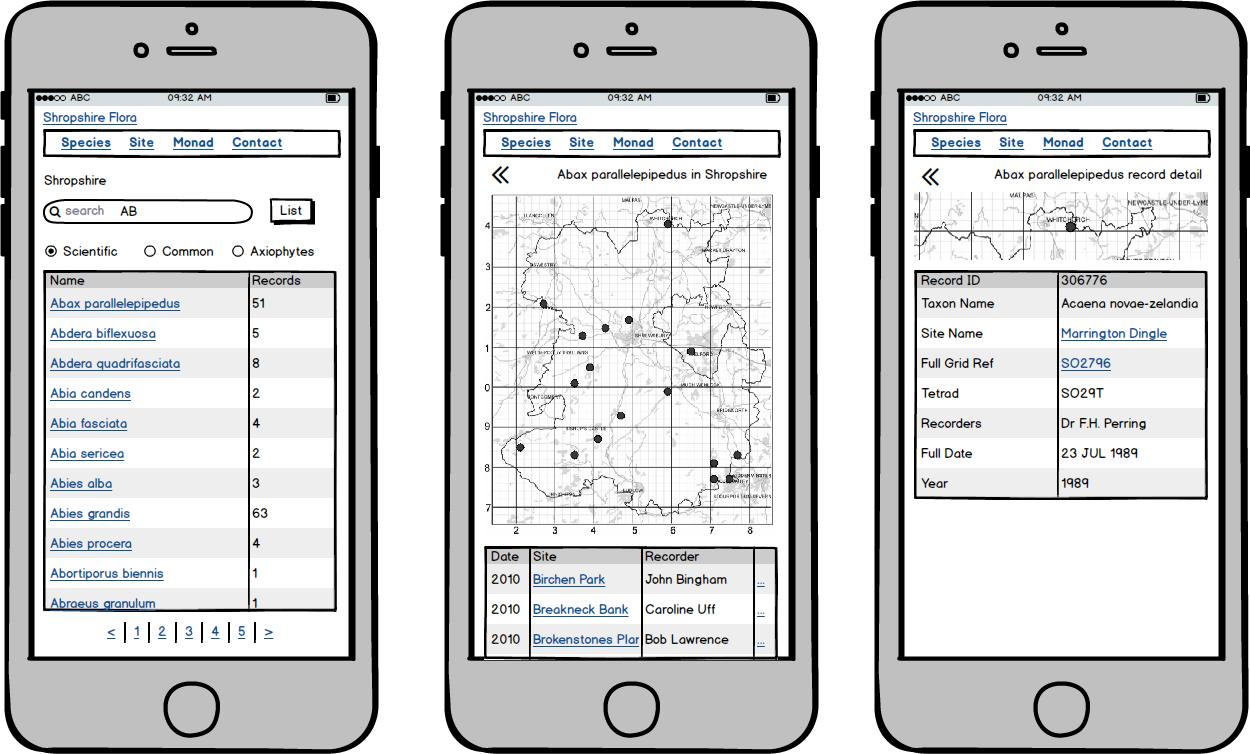
\includegraphics[width=0.85\textwidth]{./wireframes/county-mobile.png}%
\clearpage

\subsubsection{Mobile Species Search}
The `landing' page for the application is the search of the entire dataset for the county.

\begin{itemize}
  \item By default the \textbf{Scientific} name selected first.
  \item On landing the selected list is empty.
  \item The characters entered in the search box are used to search for names begining with those letters,
    not within the names.
  \item Clicking on \textbf{list} or pressing return on the desktop list will fill the list.
  \item If \textbf{Common} is selected, only the species with common names will be searched and shown.
  \item If \textbf{Axiophytes} a limited static list of scientific names will be searched and shown.
  \item Changing the radio button will reset the search and blank the list.
\end{itemize}

e.g. \url{https://records-ws.nbnatlas.org/explore/group/Plants?fq=data_resource_uid:dr782+AND+taxon_name:B*} 

\subsubsection{Mobile Species Dot Map}
Clicking on a species name will show details for the 

\begin{itemize}
  \item Collapse the map? Retain state in cookie
  \item Page the records?
  \item Site link goes to what?
\end{itemize}

\subsubsection{Mobile Sighting Record}
  
\end{multicols*}

\subsection{Desktop}
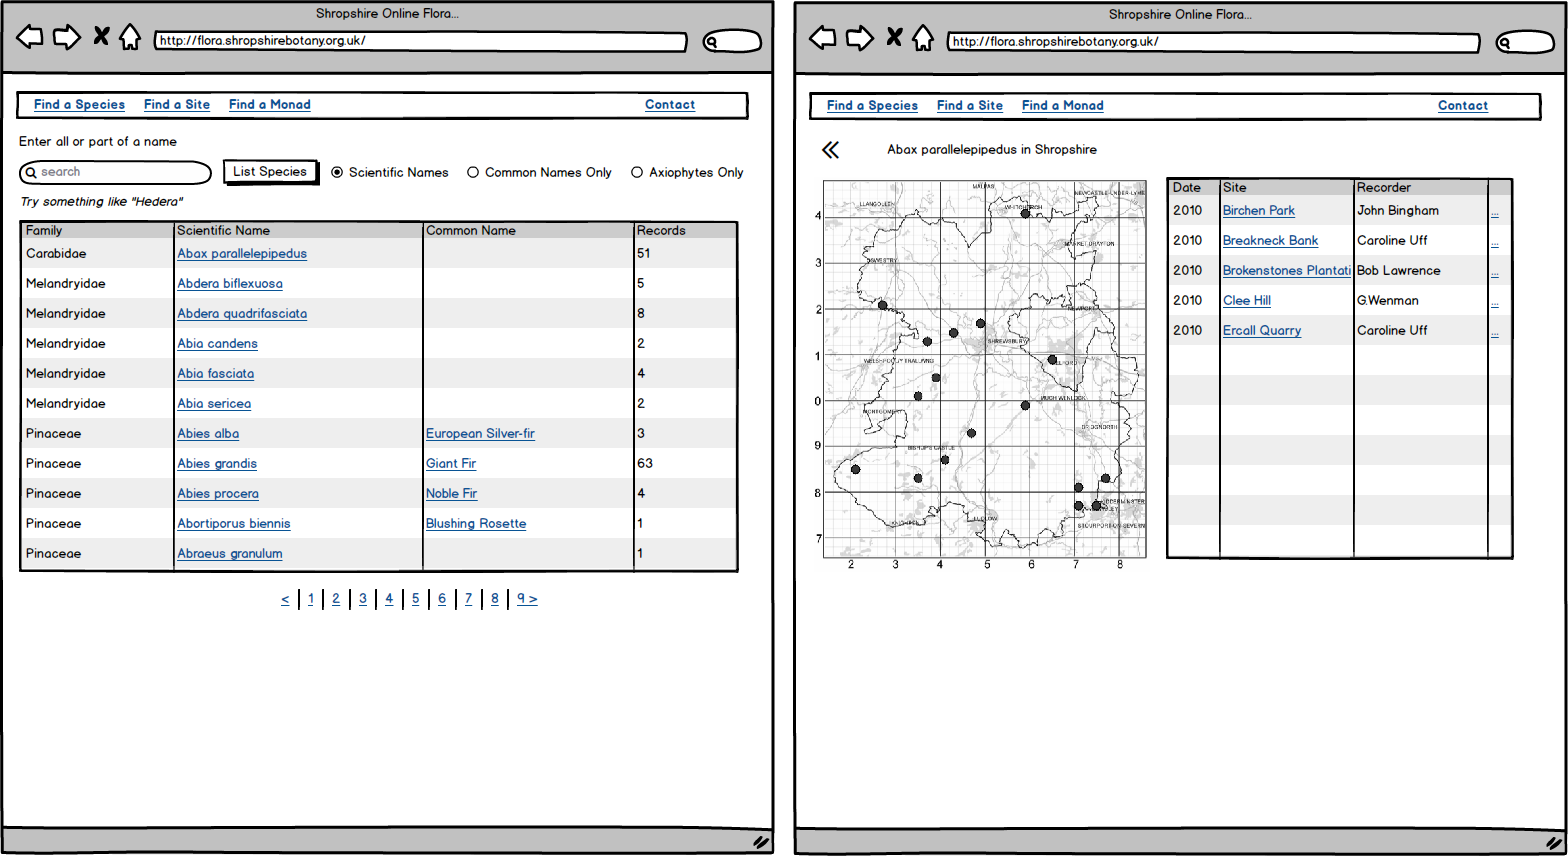
\includegraphics[width=\textwidth]{./wireframes/county-desktop.png}

\subsubsection{Desktop Species Search}

\subsubsection{Desktop Species Dot Map}

\begin{itemize}
  \item Map does not collapse.
\end{itemize}
\clearpage

\begin{multicols*}{2}[%
  \section{Search by Site}%
  \subsection{Mobile}%
]
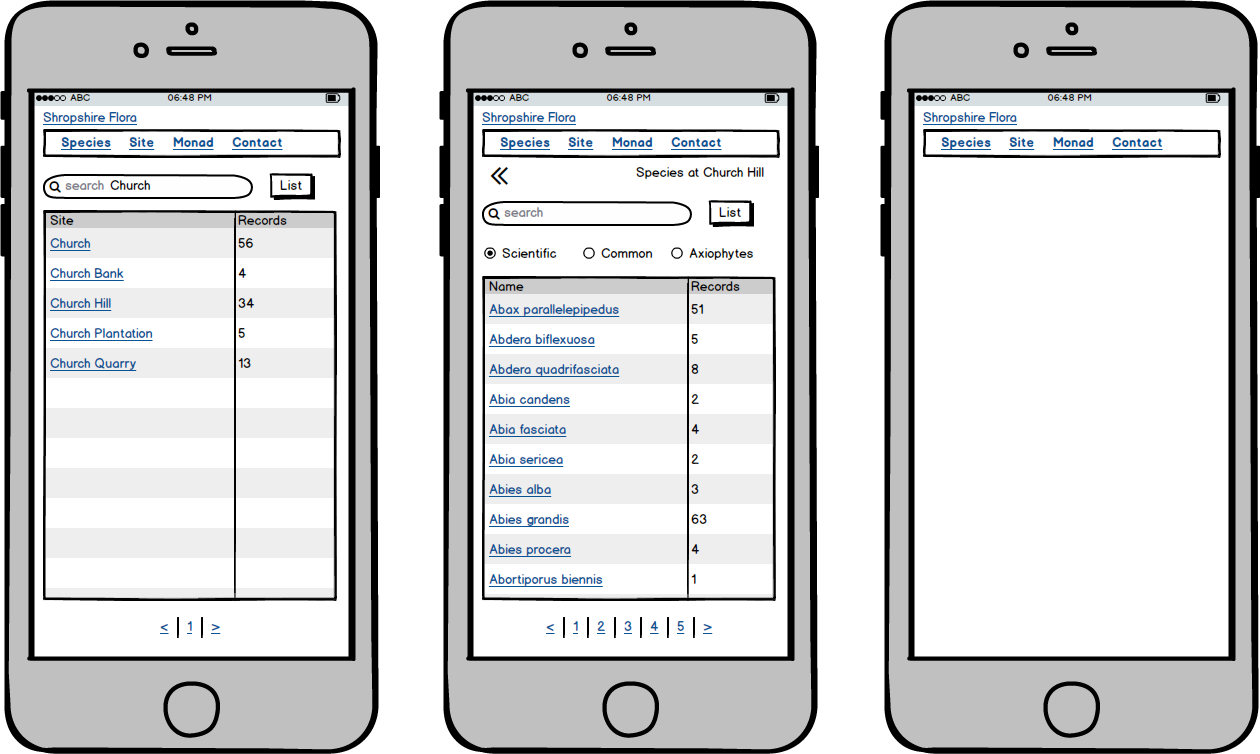
\includegraphics[width=0.85\textwidth]{./wireframes/site-mobile.png}%
\clearpage

\subsubsection{Site Search}

\begin{itemize}
  \item On landing the site list is empty.
\end{itemize}

e.g. \url{https://records-ws.nbnatlas.org/occurrences/search?fq=location_id:[Church%20TO%20*]&fq=data_resource_uid:dr782&facets=location_id&facet=on&pageSize=0}

\end{multicols*}
\clearpage

\section{Search Grid Square by Plant Name}
\subsection{Mobile}
  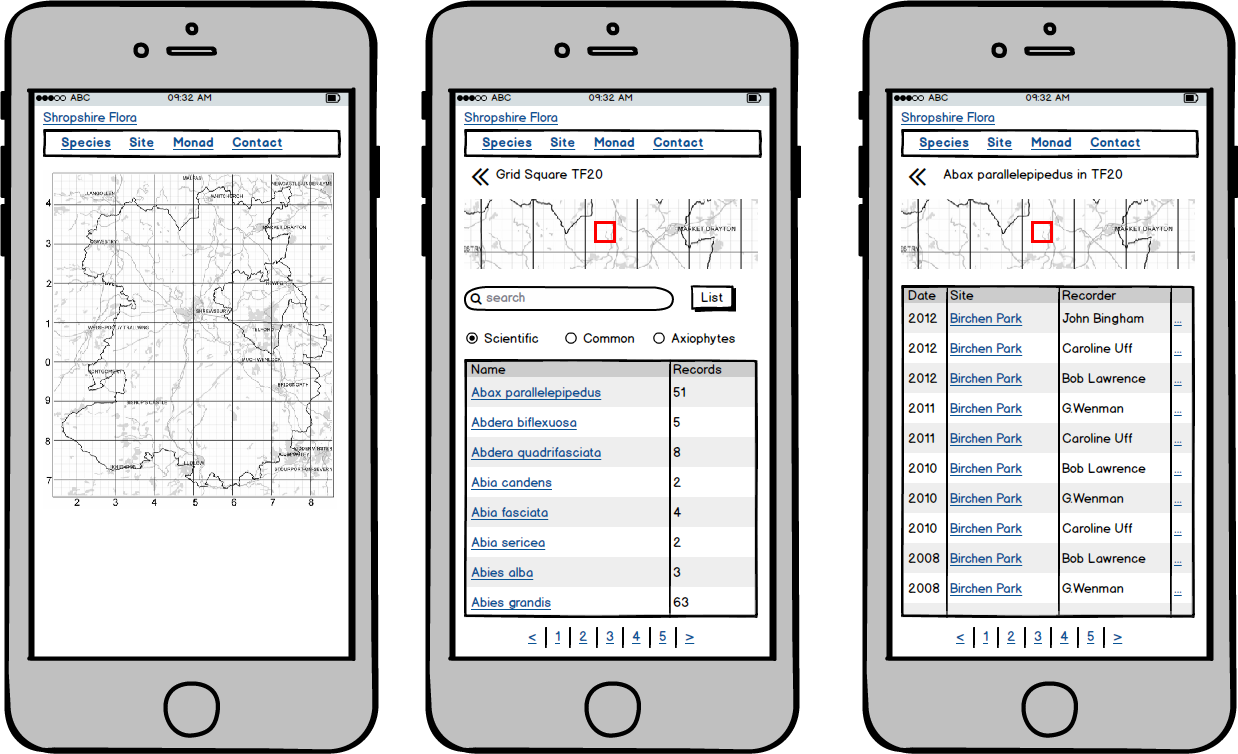
\includegraphics[width=0.85\textwidth]{./wireframes/monad-mobile.png}


\section{Technical Constraints}

% Simple and convenient caching.
% Possible to source PHP developers from within the ranks of members.
% Possibility of free hosting on the Google App Engine.
% Simplest possible with the lowest barrier to entry.
% Almost any programmer should be able to work on it.

The Botanical Society has limited means
and wishes to ensure that the results of any programming effort
can be maintained and supported
into the future.

\begin{description}
    \item[PHP 7.3] for deployment to Google App Engine.
    \item[CodeIgniter 4.0.4] has been used successfully in the past and provides convenient caching should it be required.
    \item[Twitter Bootstrap 4.5.2] for responsive layout.
    \item[Leaflet 1.6.0] should be used to provide mapping services.
     https://github.com/DuncanRowland/NBNMapOverlayExamples
    \item[Commits to Github] since the Society will retain the intellectual property rights
      over any code produced.
      So all branching should be on the repository at
      at \href{https://github.com/joejcollins/captain-magenta.git}{Github}
      The Society will
    \item[Style Sheet] taken from \href{https://www.shropshirebotany.org.uk/}{www.shropshirebotany.org.uk}.
      The Online Flora is to be consistent with this website,
      so should reuse the same classes and styles.
    \item[No API Calls from the Client] because we might want to use caching.
    \item[No database] should be used other than the NBN Web service API.
      Any static data 
      (such as the list of Axiophytes)
      should be hard coded into the application.
\end{description}





\end{document}


